% Appendix Template
\chapter{Appendix} % Main appendix title
\label{appA} % Change X to a consecutive letter; for referencing this appendix elsewhere, use \ref{AppendixX}
\begin{figure}[tbh!]
\centering
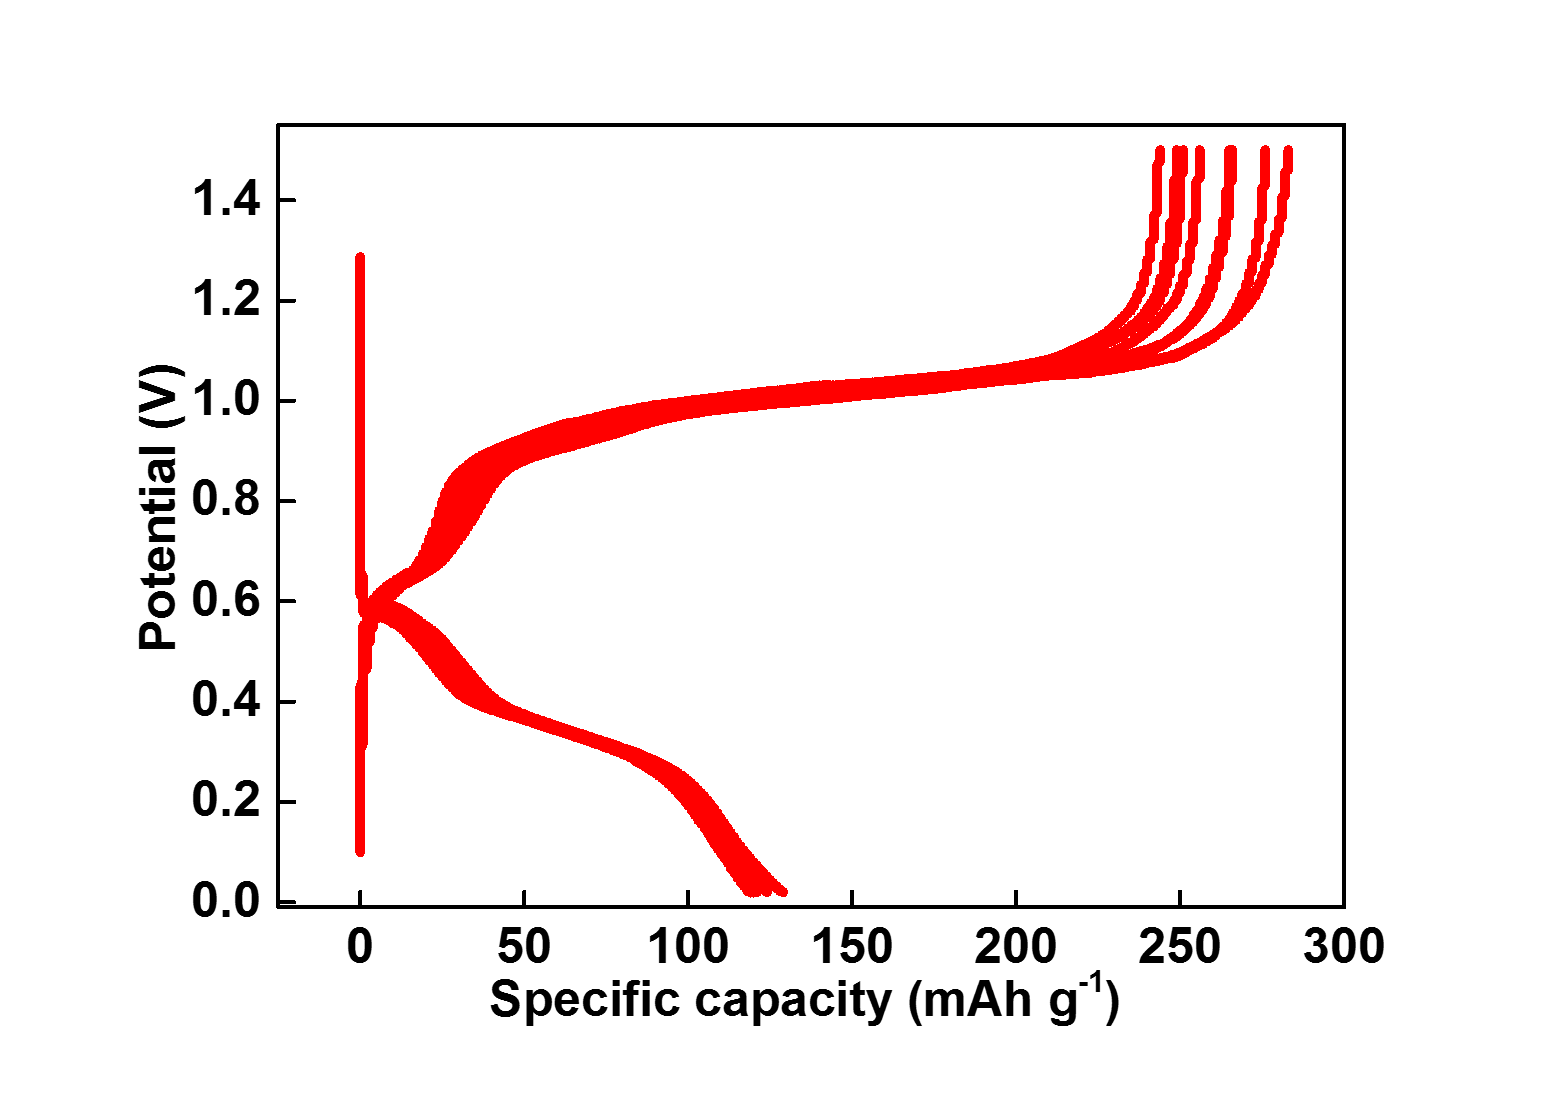
\includegraphics[width=\textwidth]{Figures/appendix/hBNrepeat}
\caption{Honeycomb lattice of a) natural graphite and b) hexagonal boron nitride. They have similar interlayer distance of 3.3\AA.}
\label{Figures/appendix:hBNrepeat}
\end{figure}
\begin{figure}[tbh!]
\centering
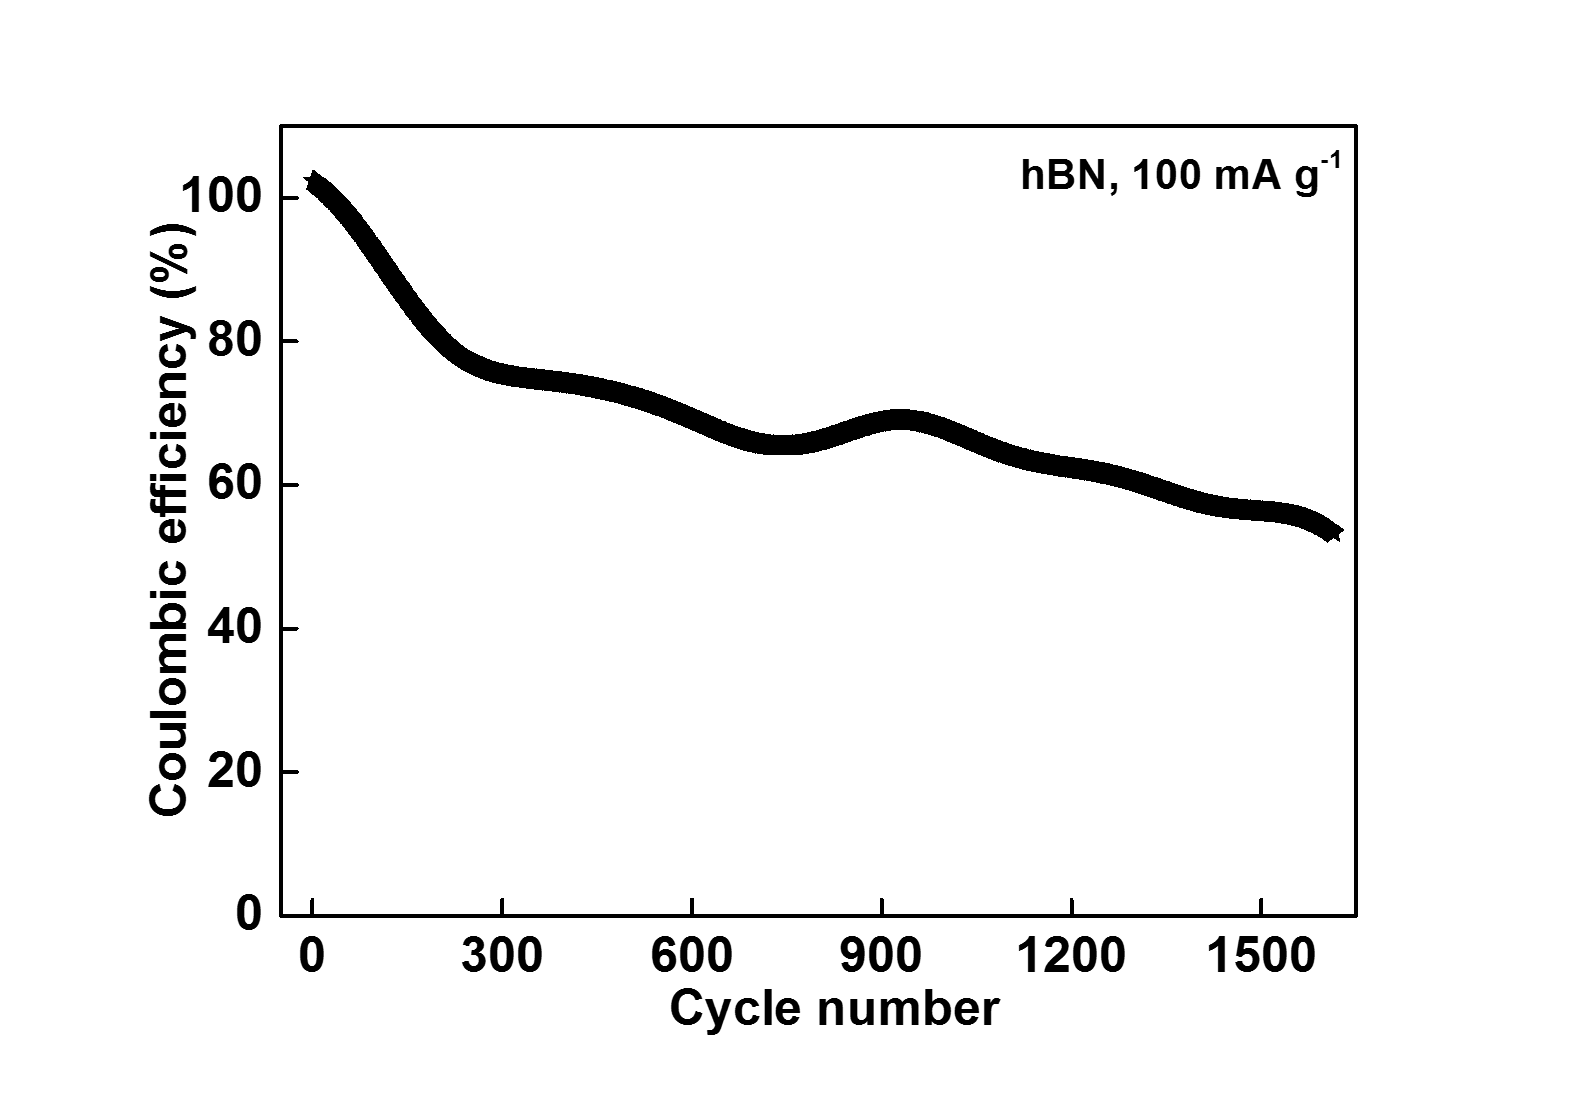
\includegraphics[width=\textwidth]{Figures/appendix/pouchCE}
\caption{a) Coulombic efficiency recorded for 1600 cycles of an Al/hBN pouch cell assembled in IKTS, Germany.}
\label{Figures/appendix:pouchCE}
\end{figure}
\begin{figure}[tbh!]
\centering
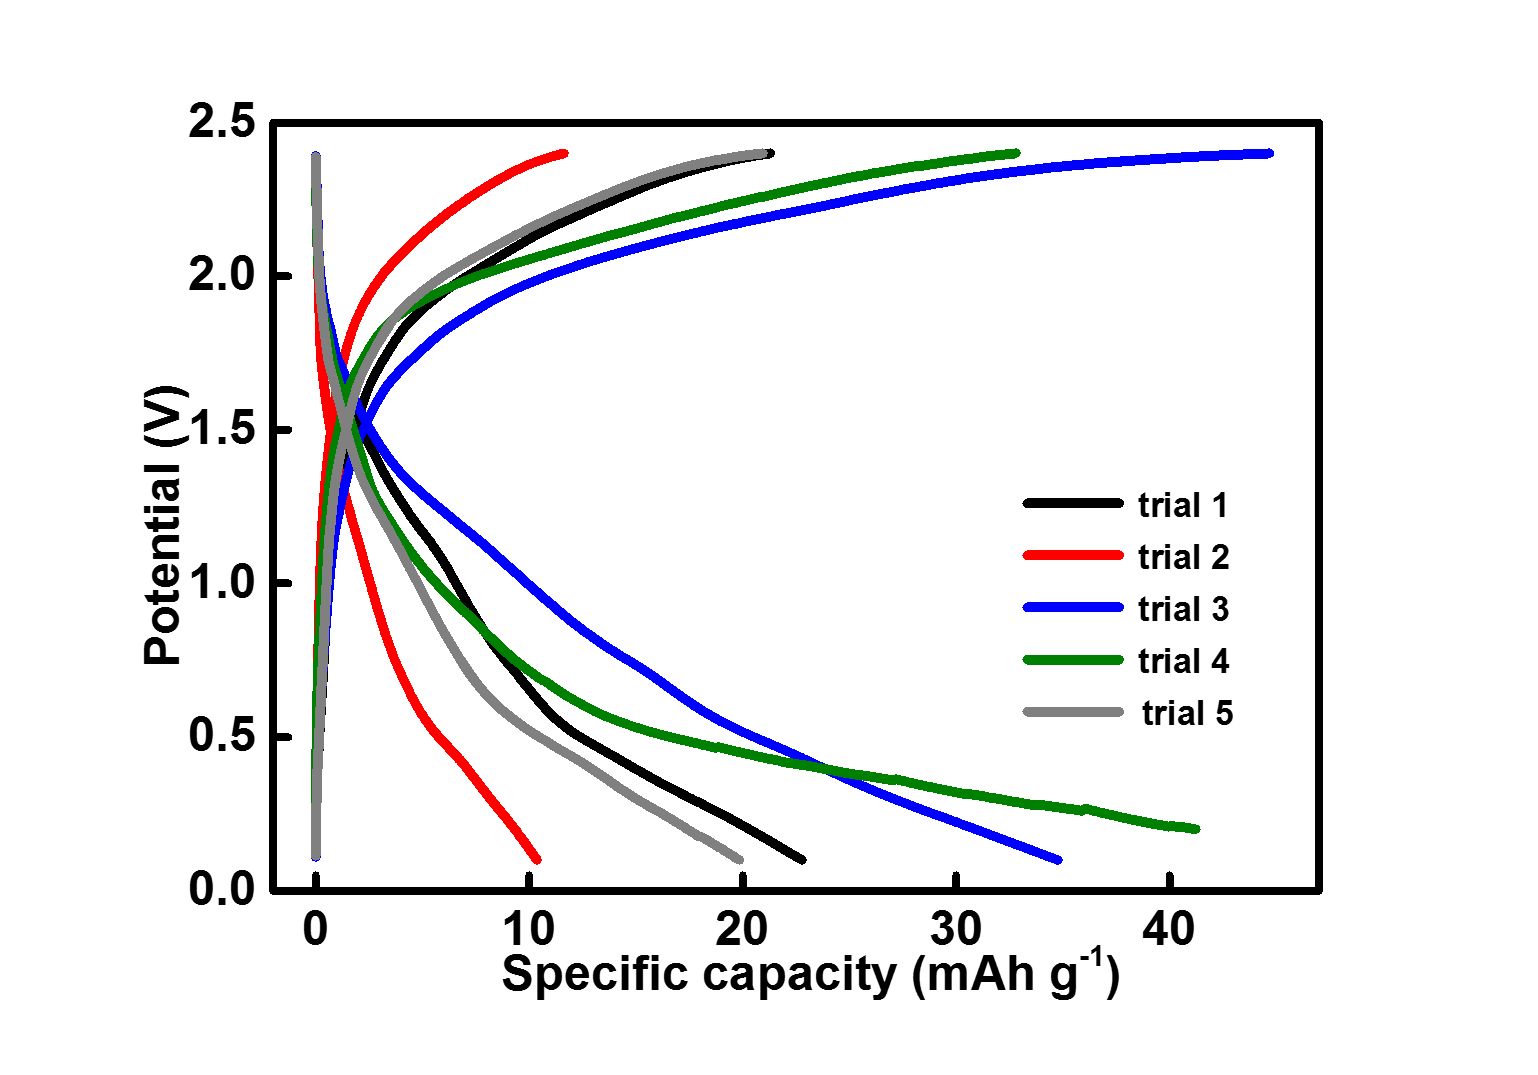
\includegraphics[width=\textwidth]{Figures/appendix/hBNmultiattempts}
\caption{a) Coulombic efficiency recorded for 1600 cycles of an Al/hBN pouch cell assembled in IKTS, Germany.}
\label{Figures/appendix:hBNmultiattempts}
\end{figure}
\begin{figure}[tbh!]
\centering
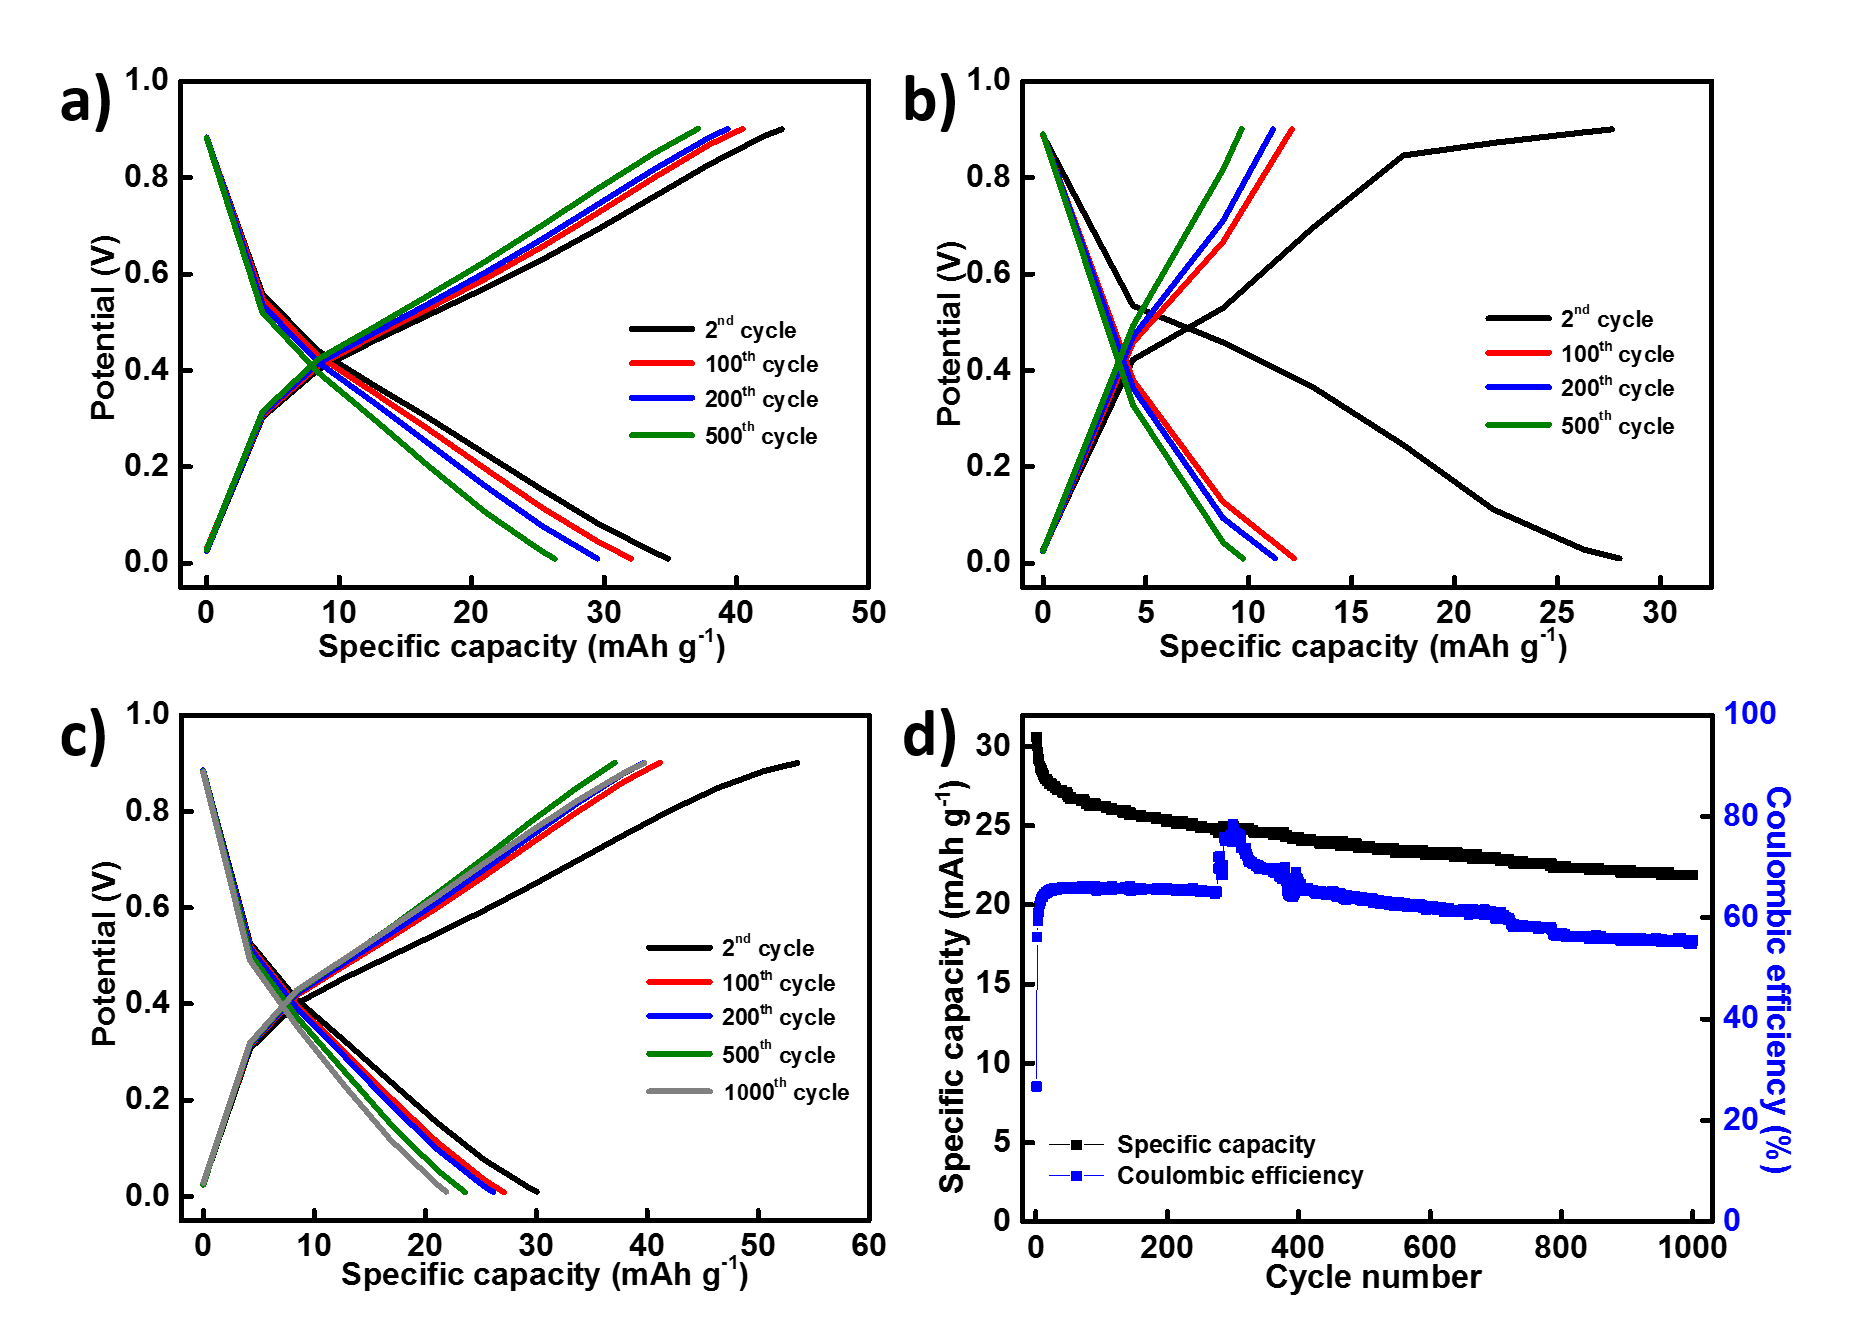
\includegraphics[width=\textwidth]{Figures/appendix/pouchcellCDCCE}
\caption{a) Coulombic efficiency recorded for 1600 cycles of an Al/hBN pouch cell assembled in IKTS, Germany.}
\label{Figures/appendix:pouchcellCDCCE}
\end{figure}